\section{Experiments Supplement}\label{sec:experiments_supplement}

\subsection{Relational Games (\Cref{ssec:exp_relational_games})}

The pentominoes split is used for training, and the hexominoes and stripes splits are used to test out-of-distribution generalization after training. We hold out 1000 samples for validation (during training) and 5000 samples for testing (after training), and use the rest as the training set. We train for 50 epochs using the categorical cross-entropy loss and the Adam optimizer with learning rate $0.001$, $\beta_1 = 0.9, \beta_2 = 0.999, \epsilon = 10^{-7}$. We use a batch size of 512. For each model and task, we run 5 trials with different random seeds.\Cref{tab:relational_games_tasks} contains text descriptions of each task in the relational games dataset in the experiments of~\Cref{ssec:exp_relational_games}.~\Cref{tab:relgames_architectures} contains a description of the architectures of each model (or shared component) in the experiments.
\Cref{tab:ood_generalization} reports the accuracy on the hold-out object sets (i.e., the numbers depicted in~\Cref{fig:ood_generalization} of the main text).~\Cref{fig:groupattn_entropy_reg} explores the effect of entropy regularization in group attention on learning using the ``match pattern'' task as an example.


\subsection{SET (\Cref{ssec:experiments_set})}

We train for 100 epochs using the categorical cross-entropy loss and the Adam optimizer with learning rate $0.001$, $\beta_1 = 0.9, \beta_2 = 0.999, \epsilon = 10^{-7}$. We use a batch size of 512. For each model and task, we run 5 trials with different random seeds.\Cref{tab:set_architectures} contains a description of the architecture of each model in the ``contains set'' experiments of~\Cref{ssec:experiments_set}.~\Cref{tab:set_acc} reports the generalization accuracies on the hold-out `sets' (i.e., the numbers depicted in~\Cref{fig:contains_set_acc} of the main text).

\begin{table}[H]
    \centering
    \begin{tabular}{p{0.2\textwidth}p{0.7\textwidth}}
    \toprule
    Task              & Description                                                                                                                                                                                             \\ \midrule
    \texttt{same}              & Two random cells out of nine are occupied by an object. They are the ``same'' if they have the same color, shape, and orientation (i.e., identical image)                                               \\\hline
    \texttt{occurs}            & The top row contains one object and the bottom row contains three objects. The ``occurs'' relationship holds if at least one of the objects in the bottom row is the same as the object in the top row. \\\hline
    \texttt{xoccurs}           & Same as occurs, but the relationship holds if exactly one of the objects in the bottom row is the same as the object in the top row.                                                                    \\\hline
    \texttt{between}           & The grid is occupied by three objects in a line (horizontal or vertical). The ``between'' relationship holds if the outer objects are the same.                                                         \\\hline
    \texttt{row match pattern} & The first and third rows of the grid are occupied by three objects each. The ``match pattern'' relationship holds if the relation pattern in each row is the same (e.g., AAA, AAB, ABC, etc.)           \\ \bottomrule
\end{tabular}
    \caption{Relational games tasks.}\label{tab:relational_games_tasks}
\end{table}

\begin{table}[H]
    \centering
    \begin{tabular}{p{0.25\textwidth}p{0.75\textwidth}}
    \toprule
    Model / Component & Architecture \\ \midrule
    Common CNN \newline Embedder & \texttt{Conv2D} $\to$ \texttt{MaxPool2D} $\to$ \texttt{Conv2D} $\to$ \texttt{MaxPool2D} $\to$ \texttt{Flatten}. \newline
                        \texttt{Conv2D}: num filters = 16, filter size = $3 \times 3$, activation = relu. \newline
                        \texttt{MaxPool2D}: stride = 2. \\\hline
    RelConvNet        & \texttt{CNN} $\to$ \texttt{MD-IPR} $\to$ \texttt{RelConv} $\to$ \texttt{Flatten} $\to$ \texttt{MLP}. \newline
                        \texttt{MD-IPR}: relation dim = 16, projection dim = 4, symmetric. \newline
                        \texttt{RelConv}: num filters = 16, filter size = 3, discrete groups = combinations. \\\hline
    CoRelNet          & \texttt{CNN} $\to$ \texttt{CoRelNet} $\to$ \texttt{Flatten} $\to$ \texttt{MLP}. \newline
                        Standard CoRelNet has no hyperparameters. \\\hline
    PrediNet          & \texttt{CNN} $\to$ \texttt{PrediNet} $\to$ \texttt{Flatten} $\to$ \texttt{MLP}. \newline
                        \texttt{PrediNet}: key dim = 4, number of heads = 4, num relations = 16. \\\hline
    Transformer       & \texttt{CNN} $\to$ \texttt{TransformerEncoder} $\to$ \texttt{AveragePooling} $\to$ \texttt{MLP}. \newline
                    \texttt{TransformerEncoder}: num layers = 1, num heads = 8, feedforward intermediate size = 32, activation = relu. \\\hline
    GCN               &
        \texttt{CNN} $\to$ \texttt{AddPosEmb} $\to$ (\texttt{GCNConv} $\to$ \texttt{Dense}) $\times 2$ $\to$ \texttt{AveragePooling} $\to$ \texttt{MLP}. \newline
        \texttt{GCConv}: channels = 128, \texttt{Dense}: num neurons = 128, activation = relu \\\hline
    GAT               &
        \texttt{CNN} $\to$ \texttt{AddPosEmb} $\to$ (\texttt{GATConv} $\to$ \texttt{Dense}) $\times 2$ $\to$ \texttt{AveragePooling} $\to$ \texttt{MLP}. \newline
        \texttt{GATonv}: channels = 128, \texttt{Dense}: num neurons = 128, activation = relu \\\hline
    GCN               &
        \texttt{CNN} $\to$ \texttt{AddPosEmb} $\to$ (\texttt{GINConv} $\to$ \texttt{Dense}) $\times 2$ $\to$ \texttt{AveragePooling} $\to$ \texttt{MLP}. \newline
        \texttt{GINConv}: channels = 128, \texttt{Dense}: num neurons = 128, activation = relu \\\hline
                Common output MLP & \texttt{Dense(64, `relu')} $\to$ \texttt{Dense(2)}. \\ \bottomrule
\end{tabular}
    \caption{Model architectures for relational games experiments.}\label{tab:relgames_architectures}
\end{table}

\begin{table}[H]
    \centering
    \begin{tabular}{llll}
\toprule
              &             &     Hexos Accuracy &   Stripes Accuracy \\
Task & Model &                    &                    \\
\midrule
same & RelConvNet &  $0.989 \pm 0.002$ &  $0.974 \pm 0.003$ \\
              & CoRelNet &  $0.988 \pm 0.006$ &  $0.724 \pm 0.112$ \\
              & PrediNet &  $0.990 \pm 0.004$ &  $0.983 \pm 0.007$ \\
              & Transformer &  $0.997 \pm 0.001$ &  $0.993 \pm 0.004$ \\\hline
occurs & RelConvNet &  $0.980 \pm 0.001$ &  $0.880 \pm 0.015$ \\
              & CoRelNet &  $0.992 \pm 0.004$ &  $0.518 \pm 0.012$ \\
              & PrediNet &  $0.907 \pm 0.020$ &  $0.775 \pm 0.046$ \\
              & Transformer &  $0.881 \pm 0.015$ &  $0.724 \pm 0.021$ \\\hline
xoccurs & RelConvNet &  $0.967 \pm 0.001$ &  $0.946 \pm 0.006$ \\
              & CoRelNet &  $0.980 \pm 0.007$ &  $0.606 \pm 0.035$ \\
              & PrediNet &  $0.872 \pm 0.036$ &  $0.810 \pm 0.028$ \\
              & Transformer &  $0.867 \pm 0.017$ &  $0.753 \pm 0.031$ \\\hline
between & RelConvNet &  $0.991 \pm 0.001$ &  $0.988 \pm 0.002$ \\
              & CoRelNet &  $0.995 \pm 0.001$ &  $0.582 \pm 0.063$ \\
              & PrediNet &  $0.978 \pm 0.006$ &  $0.950 \pm 0.019$ \\
              & Transformer &  $0.986 \pm 0.003$ &  $0.961 \pm 0.010$ \\\hline
match pattern & RelConvNet &  $0.961 \pm 0.015$ &  $0.870 \pm 0.041$ \\
              & CoRelNet &  $0.942 \pm 0.011$ &  $0.581 \pm 0.026$ \\
              & PrediNet &  $0.710 \pm 0.040$ &  $0.658 \pm 0.053$ \\
              & Transformer &  $0.627 \pm 0.005$ &  $0.591 \pm 0.006$ \\
\bottomrule
\end{tabular}

    \caption{Out-of-distribution generalization results on relational games. We report means $\pm$ standard error of mean over 5 trials. These are the numbers associated with~\Cref{fig:ood_generalization}.}\label{tab:ood_generalization}
\end{table}

\begin{table}[H]
    \centering
    \begin{tabular}{p{0.25\textwidth}p{0.75\textwidth}}
    \toprule
    Model / Component & Architecture                                                                                                                                                                                                                                                                                       \\ \midrule
    Common CNN \newline Embedder & 
        \texttt{Conv2D} $\to$ \texttt{MaxPool2D} $\to$ \texttt{Conv2D} $\to$ \texttt{MaxPool2D} $\to$ \texttt{Flatten} $\to$ \texttt{Dense(64, 'relu') $\to$ \texttt{Dense(64, 'tanh')}}. \newline
        \texttt{Conv2D}: num filters = 32, filter size = $5 \times 5$, activation = relu. \newline
        \texttt{MaxPool2D}: stride = 4. \\\hline
    RelConvNet        & 
        \texttt{CNN} $\to$ \texttt{MD-IPR} $\to$ \texttt{RelConv} $\to$ \texttt{Flatten} $\to$ \texttt{MLP}. \newline
        \texttt{MD-IPR}: relation dim = 16, projection dim = 16, symmetric. \newline
        \texttt{RelConv}: num filters = 16, filter size = 3, discrete groups = combinations, symmetric relational inner product with `max' aggregator. \\\hline
    CoRelNet          &
        \texttt{CNN} $\to$ \texttt{CoRelNet} $\to$ \texttt{Flatten} $\to$ \texttt{MLP}. \newline
        Standard CoRelNet has no hyperparameters. \\\hline
    PrediNet          &
        \texttt{CNN} $\to$ \texttt{PrediNet} $\to$ \texttt{Flatten} $\to$ \texttt{MLP}. \newline
        \texttt{PrediNet}: key dim = 4, number of heads = 4, num relations = 16. \\\hline
    Transformer       & 
        \texttt{CNN} $\to$ \texttt{TransformerEncoder} $\to$ \texttt{AveragePooling} $\to$ \texttt{MLP}. \newline
        \texttt{TransformerEncoder}: num layers = 1, num heads = 8, feedforward intermediate size = 32, activation = relu. \\\hline
    GCN               &
        \texttt{CNN} $\to$ (\texttt{GCNConv} $\to$ \texttt{Dense}) $\times 2$ $\to$ \texttt{AveragePooling} $\to$ \texttt{MLP}. \newline
        \texttt{GCConv}: channels = 128, \texttt{Dense}: num neurons = 128, activation = relu \\\hline
    GAT               &
        \texttt{CNN} $\to$ (\texttt{GATConv} $\to$ \texttt{Dense}) $\times 2$ $\to$ \texttt{AveragePooling} $\to$ \texttt{MLP}. \newline
        \texttt{GATonv}: channels = 128, \texttt{Dense}: num neurons = 128, activation = relu \\\hline
    GCN               &
        \texttt{CNN} $\to$ (\texttt{GINConv} $\to$ \texttt{Dense}) $\times 2$ $\to$ \texttt{AveragePooling} $\to$ \texttt{MLP}. \newline
        \texttt{GINConv}: channels = 128, \texttt{Dense}: num neurons = 128, activation = relu \\\hline
    Common output MLP & \texttt{Dense(64, `relu')} $\to$ \texttt{Dense(32, `relu')} $\to$ \texttt{Dense(2)}. \\ \bottomrule
\end{tabular}
    \caption{Model architectures for ``contains set'' experiments.}\label{tab:set_architectures}
\end{table}

\begin{figure}[H]
    \centering
    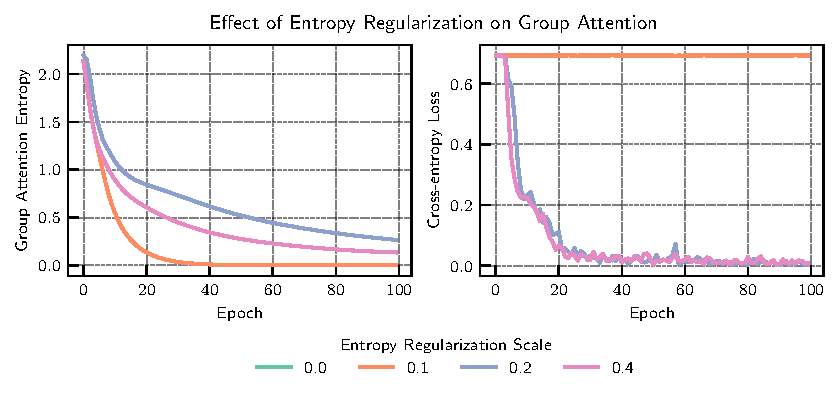
\includegraphics{figs/experiments/group_attn_entropy.pdf}
    \caption{Effect of group attention entropy regularization. Group attention entropy (left) and baseline cross-entropy loss (right) of a relational convolutional network model trained on the ``match pattern'' task with different levels of entropy regularization. The overall model loss is $\calL_{\mathtt{loss}} + \lambda \calL_{\mathtt{entr}}$, where $\calL_{\mathtt{loss}} = \mathrm{CrossEntropy}(y, \hat{y})$, $\calL_{\mathtt{entr}}$ is the entropy regularization term for the group attention scores as defined in~\Cref{ssec:relconv_groupattn}, and $\lambda$ is a scaling factor. Different lines correspond to different values of $\lambda$. Without entropy regularization, the model fails to learn the task. With sufficient entropy regularization, the model is able to learn the task and group attention converges towards discrete assignments. The group attention entropy starts at $\log 9 \approx 2.2$ (the entropy of a uniform distribution) and decreases over the course of training.}\label{fig:groupattn_entropy_reg}
\end{figure}

\aafatal{TODO -- add additional trials. add further discussion}

\begin{table}[H]
    \centering
    \begin{tabular}{ll}
\toprule
{} &           Accuracy \\
Model       &                    \\
\midrule
RelConvNet  &  $0.979 \pm 0.006$ \\
CoRelNet    &  $0.563 \pm 0.001$ \\
PrediNet    &  $0.508 \pm 0.002$ \\
Transformer &  $0.584 \pm 0.004$ \\
GCN         &  $0.595 \pm 0.003$ \\
GAT         &  $0.517 \pm 0.015$ \\
GIN         &  $0.590 \pm 0.003$ \\
LSTM        &  $0.602 \pm 0.003$ \\
GRU         &  $0.593 \pm 0.004$ \\
\bottomrule
\end{tabular}

    \caption{Hold-out test accuracy on ``contains set'' task. We report means $\pm$ standard error of mean over 10 trials. These are the numbers associated with~\Cref{fig:contains_set_acc}.}\label{tab:set_acc}
\end{table}
\null
\vfill
